% Definimos el estilo del documento
\documentclass[12pt,a4paper,spanish]{book}

\usepackage[utf8]{inputenc}
\usepackage[english,spanish]{babel}
\usepackage{ amssymb }
\usepackage{ amsmath }
\usepackage{ amsthm }
\usepackage{ wasysym }
\usepackage{ verbatim }
\usepackage{ fancyvrb }
\usepackage{ url }
\usepackage[table]{xcolor}% http://ctan.org/pkg/xcolor
\usepackage{ tikz }
\usetikzlibrary{shapes.gates.logic.US,trees,positioning,arrows,shapes.multipart,snakes}


\usepackage{ appendix }
\renewcommand{\appendixname}{Apéndices}
\renewcommand{\appendixtocname}{Apéndices}
\renewcommand{\appendixpagename}{Apéndices}
\newcommand{\frob}{Willie}
\newcommand{\alf}{Alf}
\newcommand{\compilador}{\texttt{williec}}
\newcommand{\maquinavirtual}{Alfvm}
 
%\usepackage[dvips]{graphicx}
%\DeclareGraphicsExtensions{.pdf,.png,.jpg}

\usepackage{graphicx}

\usepackage{hyperref}
\hypersetup{colorlinks=false}

\usepackage{proof}

\newtheorem{definicion}{Definición}

%Empieza el documento
\begin{document}
\selectlanguage{spanish}

% Definimos titulo, autor, fecha.
\title{
  \frob: Programación funcional reactiva para robots con bajas capacidades de cómputo\\
    {\small Proyecto de grado, Facultad de Ingeniería, Universidad de la República}\\
  \begin{center}
    {
\includegraphics[width=40mm]{fing.jpg}}
    {
\includegraphics[width=40mm]{udelar.jpg}}
  \end{center}
}
\author{Guillermo Pacheco\\
{\small Tutores: Marcos Viera, Jorge Visca, Andrés Aguirre}}
\date{\today}

% Generamos titulo e indice de contenidos
\maketitle


% Resumen
\chapter*{Resumen}
\addcontentsline{toc}{chapter}{Resumen}
\markboth{RESUMEN}{RESUMEN}


El proyecto consiste en la creación de un lenguaje de programación
para robots, cuyas capacidades de cómputo son limitadas.
Para esto se escogió el paradigma de Programación Funcional Reactiva
(\emph{FRP}) el cual permite expresar naturalmente reacciones a
valores que varían en función del tiempo.

El objetivo es utilizarlo con fines educativos,
por lo tanto debe ser simple y fácil de usar por usuarios
inexpertos, no familiarizados con la electrónica ni la informática.

Para resolver el problema, se dividió en dos etapas.

La primera consiste en la implementación de
un compilador que traduce el lenguaje cuyo nivel es alto a
un lenguaje de bajo nivel (\emph{Bytecode}) más simple e interpretable.

La segunda etapa consiste en implementar una máquina virtual, que
sea capaz de interpretar el lenguaje de bajo nivel.
Por cada plataforma objetivo, es posible realizar una implementación de
la máquina, lo que permite ejecutar los mismos
programas en alto nivel, en diferentes plataformas.

El diseño de la máquina consiste de un núcleo común capaz de interpretar
instrucciones, y módulos bien definidos de
entrada/salida los cuáles varían de una plataforma a otra.
Ésto permite mayor portabilidad y extensibilidad.

Debe ser posible ejecutar programas en dicho lenguaje dentro de plataformas
de hardware reducido.
Considerando ésto, el lenguaje de programación elegido para la
implementación de la máquina virtual es C/C++.

De esta forma se implementó un lenguaje reactivo con las
características deseadas, y una implementación modelo de una máquina
virtual que permite
su ejecución en una arquitectura objetivo deseada.
La misma es fácil de mantener, portable y cuenta con suficiente
flexibilidad para ser extendida.



% Indice general
\cleardoublepage
\addcontentsline{toc}{chapter}{Índice general} % para que aparezca en el indice de contenidos
\tableofcontents

% Indice de figuras
\cleardoublepage
\addcontentsline{toc}{chapter}{Índice de figuras} % para que aparezca en el indice de contenidos
\listoffigures

% indice de tablas
\cleardoublepage
\addcontentsline{toc}{chapter}{Índice de tablas} % para que aparezca en el indice de contenidos
\listoftables

\chapter{Introducción}
En este capítulo se realiza una introducción a la Lógica Temporal Lineal, como una extensión de Lógica 
 Proposicional para poder expresar propiedades en sistemas reactivos.
Con esta finalidad, este lenguaje fue introducido por Pnueli en \cite{pnueli}.

La Lógica Lineal Temporal permite expresar propiedades sobre los sistemas en cuestón,
 ya que se agregan operadores que hacen referencia al tiempo y permite representar los distintos estados
 en distintos momentos durante la ejecución del sistema.


\chapter{Programación Funcional Reactiva}




\section{Programación Funcional Reactiva}

Acá voy a hablar de programación funcional reactiva.

Tradicionalmente los programas son formados a partir de
una secuencia de acciones imperativas. Los programas
reactivos suelen formarse por eventos y código iterativo
que se corre cuando un evento ocurre.

Dicho código iterativo suele hacer referencia y manipular
variables compartidas con diferentes rutinas. Ésto lleva a que
como un valor puede ser manipulado desde diferentes lugares,
puedan producirse problemas de concurrencia y algunos valores
pueden quedar en un estado inconsistente.

En el paradigma FRP no existen valores compartidos, sinó que
dichos valores dependientes del tiempo, tienen una representación
llamada Comportamiento y la única forma de modificarlos, es
a partir de como fueron definidos.

 

\begin{definicion}
Comportamientos (Behaviours).\\
Un comportamiento es un valor contínuo que depende del paso del tiempo.
Los comportamientos se pueden definir, combinar, pasarlos como
argumentos a funciones, retornarlos.
Un comportamiento puede ser un valor constante, el tiempo mismo (un reloj),
o puede formarse combinando otros comportamientos, por ejemplo secuencialmente
o paralelamente.
\end{definicion}

\begin{definicion}
Eventos (Streams).\\
Son valores discretos dependientes del tiempo, que forman
una secuencia finita o infinita de ocurrencias. Cada ocurrencia
está formada por el valor y el instante de tiempo.
\end{definicion}

La principal diferencia entre Comportamientos y Eventos, es que los
comportamientos son valores contínuos y los eventos son discretos.

Los comportamientos representan cualquier valor en función del tiempo,
por ejemplo:
\begin{itemize}
\item \textit{entrada} sensor de distancia, temperatura, video
\item \textit{salida} velocidad, voltaje
\item \textit{valores} intermedios calculados
\end{itemize}

Las operaciones que se pueden realizar sobre los comportamientos incluyen:
\begin{itemize}
\item \textit{Operaciones genéricas} Aritmética, integración, diferenciación
\item \textit{Operaciones específicas de un dominio} como escalar video, aplicar filtros, detección de patrones.
\end{itemize}

Los eventos pueden ser sensores específicos de un dominio, por ejemplo un
botón, un click, una interrupción o mensaje asincrónico.
También puede ser generado a partir de valores de un comportamiento,
como ser \emph{Temperatura alta}, \emph{Batería baja}.

Las operaciones que se pueden realizar sobre los eventos incluyen:
\begin{itemize}
\item fmap, filter
\item Modificar un \emph{Comportamiento} reactivo
\end{itemize}


\section{Ejemplo}

Para entender un poco más las ideas de Comportamiento y Evento, se puede
plantear el siguiente ejemplo.

  En una cuenta de un banco, el saldo se puede definir
como un comportamiento, el cuál solo se modifica cuando ocurre
un movimiento.
  Un movimiento puede ser depositar dinero o extraer
dinero de la cuenta.
  Un dato importante a ver, es que no es posible asignar un valor
sin que sea por medio de su propia definición, por lo que nadie
podría realizar la asignación $saldo = 1000000$.
  La misma operación sería posible creando un movimiento, el cuál
afectaría al saldo.

  Usaremos la notación $<nombre> :: Event <tipo>$ para definir
eventos y la notación $<nombre> :: Behaviour <tipo>$ para
definir comportamientos.

\begin{verbatim}
movimiento :: Event Number
movimiento = read(0)

saldo :: Behaviour Number
saldo = movimiento

alert :: Event Bool
alert = saldo > 1000

on alert:
  write(0, 'El saldo es mayor a 1000')

\end{verbatim}

Un comportamiento, solo se modifica cuando cambian sus componentes,





%state = State(state, [input])
%Output(state)


\chapter{Plataformas de Hardware}

En esta sección se describen las plataformas de hardware relevadas
durante el estado del arte, junto con sus características.

\section{Arduino}

  Arduino \cite{arduino} es una plataforma abierta de prototipado, basada en
software y hardware flexible fácil de usar.
  Está pensada para ser usada por diseñadores, artistas, como
hobby, para crear objetos y ambientes interactivos.
  Entre sus productos, hay placas y kits de componentes.
  Los kits de arduino generalmente tienen interfaz usb con soporte
para programarlo usando la propia placa sin necesidad de un
programador por hardware.

  También los pines de entrada/salida del microprocesador
están diseñados para poder colocar fácilmente cables y
conectar periféricos sin necesidad de soldar.

  Tambien incluyen leds y botones para resetear la placa o
utilizarlos como sensor.

  Existe un entorno de desarrollo integrado (IDE) que utiliza
una implementación del compilador \texttt{gcc} \cite{gcc} para la arquitectura
\texttt{avr} \cite{avr} de \textit{Atmel} \cite{atmel} y puede ser utilizado
para programar sobre los kits.

  Variedad de bibliotecas y abstracciones de sensores, actuadores y
protocolos de comunicación, ya están implementados y pueden ser
usados en los kits.
  Al ser un proyecto libre las bibliotecas son publicadas y mantenidas
por una comunidad abierta.

  La arquitectura usada por casi todos los kits
es \texttt{avr} \texttt{Atmel} pero existen algunos con
arquitectura \texttt{ARM} \cite{arm}.

  El lenguaje estándar para desarrollar programas se llama \texttt{Arduino},
sin embargo el lenguaje es \texttt{C/C++}, cambiando la forma en que
se invoca el programa principal y con algunas funciones y
formato predefinido.

  La Tabla \ref{table-arduino} muestra un listado de los modelos
de Arduino, cuánta memoria persistente tienen (Flash) en kilobytes, con
cuánta memoria RAM cuentan, cuánta memoria EEPROM tienen en kilobytes,
que procesador tienen y la frecuencia de funcionamiento.

  Salvo el modelo \texttt{Due}, el resto utilizan la
arquitectura \texttt{avr} de 8 bit. La memoria ram varía entre
16 y 512 kilobytes.
  Los modelos más populares y representativos, son el Arduino \texttt{Uno}
y el Arduino \texttt{Nano 328}, ambos con 32 KB de memoria Flash, 2 KB de memoria
RAM (SRAM) y procesador \texttt{ATmega328} a 16 MHz.

\begin{table}[htbp]
\centering
\scriptsize
\setlength\tabcolsep{2pt}
\caption{Modelos arduino}
\label{table-arduino}
\begin{tabular}{|c|c|c|c|c|c|c|}
  \hline
  Modelo & Flash & SRAM (kb) & EEPROM (kb) & Procesador & Arquitectura & Frecuencia \\
  \hline
  Uno & 32 KB & 2 & 1 & ATmega328 & 8 bit AVR & 16 MHz \\
  \hline
  Leonardo & 32 KB & 2.5 & 1 & ATmega32u4 & 8 bit AVR & 16 MHz \\
  \hline
  Due & 512 KB & 96 & - & AT91SAM3X8E & ARM Cortex-M3 & 84 Mhz \\
  \hline
  Yun & 32 KB & 2.5 & 1 & ATmega32u4 & 8 bit AVR & 16 MHz \\
  \hline
  Tre & 32 KB & 2.5 & 1 & ATmega32u4 & 8 bit AVR & 16 MHz \\
  \hline
  Micro & 32 KB & 2.5 & - & ATmega32u4 & 8 bit AVR & 16 MHz \\
  \hline
  Robot & 32 KB & 2.5 & 1 & ATmega32u4 & 8 bit AVR & 16 MHz \\
  \hline
  Esplora & 32 KB & 2.5 & 1 & ATmega32u4 & 8 bit AVR & 16 MHz \\
  \hline
  Mega ADK & 256 KB & 8 & 4 & ATmega2560 & 8 bit AVR & 16 MHz \\
  \hline
  Ethernet & 32 KB & 2 & 1 & ATmega328 & 8 bit AVR & 16 MHz \\
  \hline
Mega 2560 & 256 KB & 8 & 4 & ATmega2560 & 8 bit AVR & 16 MHz \\
  \hline
  Mini & 32 KB & 2 & 1 & ATmega328 & 8 bit AVR & 16 MHz \\
  \hline
  LilyPad USB & 32 KB & 2.5 & 1 & ATmega32u4 & 8 bit AVR & 8 Mhz \\
  \hline
  LilyPad Simple & 32 KB & 2 & 1 & ATmega328 & 8 bit AVR & 8 Mhz \\
  \hline
  LilyPad (168V) & 16 KB & 1 & 512 Bytes & ATmega168V & 8 bit AVR & 8 Mhz \\
  \hline
  LilyPad (328V) & 16 KB & 1 & 512 Bytes & ATmega328V & 8 bit AVR & 8 Mhz \\
  \hline
  Nano (168) & 16 KB & 1 & 512 Bytes & ATmega168 & 8 bit AVR & 16 MHz \\
  \hline
  Nano (328) & 32 KB & 2 & 1 & ATmega328 & 8 bit AVR & 16 MHz \\
  \hline
  Pro mini (3.3v) & 16 KB & 1 & 512 Bytes & ATmega168 & 8 bit AVR & 8 Mhz \\
  \hline
  Pro mini (5v) & 16 KB & 1 & 512 Bytes & ATmega168 & 8 bit AVR & 16 MHz \\
  \hline
  Pro (168) & 16 KB & 1 & 512 Bytes & ATmega168 & 8 bit AVR & 8 Mhz \\
  \hline
  Pro (328) & 32 KB & 2 & 1 & ATmega328 & 8 bit AVR & 16 MHz \\
  \hline
  Fio & 32 KB & 2 & 1 & ATmega328P & 8 bit AVR & 8 Mhz \\
  \hline 
\end{tabular}
\end{table}

%%\subsection{Arduino Uno}
%%Web: http://arduino.cc/en/Main/ArduinoBoardUno
%%Microcontrolador: ATmega328
%%Características generales:
%%Es una placa basada en el microcontrolador ATmega328.
%%0.5 kb de la memoria flash son utilizados por bootloader.
%%Existe una placa construida en uruguay llamada Urduino328,
%%la cuál es compatible con la Arduino Uno y tiene un costo aproximado de 50 dólares.
%%
%%\subsection{Arduino Leonardo}
%%Web:
%%http://arduino.cc/en/Main/ArduinoBoardLeonardo
%%Características generales:
%%Es una placa basada en el microcontrolador ATmega32u4. Tiene 20 pins de entrada/salida digitales, frecuencia de 16 MHz y conección micro USB.
%%La diferencia principal con otras placas es que el microcontrolador permite la comunicación usb sin necesidad de un microcontrolador secundario que la implemente.
%%Un bootloader es incluído, el cuál se puede utilizar para programar la placa sin un programador por hardware. Éste bootloader ocupa 4 kb de la memoria Flash del microcontrolador, puede ser eliminado pero teniendo en cuenta que luego no se cuenta con su funcionalidad.
%%Microcontrolador:
%%ATmega32u4
%%
%%\subsection{Arduino Due}
%%Web:
%%http://arduino.cc/en/Main/ArduinoBoardDue
%%Características:
%%Es la primer placa arduino basada en la arquitectura ARM de 32 bits.
%%Tiene 54 pins de entrada/salida digital, 12 de los cuáles pueden ser usados como salidas PWM.
%%12 entradas analógicas, un reloj de 84 MHz integrado, conección USB, 2 convertidores digital-analógico.
%%
%%Un botón de reset y un botón de borrado.
%%A diferencia de otras placas, ésta placa corre con un voltaje de 3.3V.
%%La mejora sustancial con respecto a otras placas, puede ejecutar operaciones sobre 4 bytes en un sólo ciclo de reloj,
%%tiene una frecuencia alta de reloj, 96 kbytes de SRAM, 512 kb de memoria flash para código y
%%un controlador DMA para liberar el CPU de tareas basadas en muchos accesos a memoria.
%%
%%El bootloader que incluye viene de fábrica y está en una ROM dedicada, por lo que no ocupa espacio de la memoria Flash.
%%
%%Microcontrolador: Atmel SAM3X8E ARM Cortex-M3
%%
%%\subsection{Arduino Robot}
%%Web:
%%http://arduino.cc/en/Main/Robot
%%Características:
%%Es el primer Arduino sobre ruedas oficial.
%%Cuenta con dos procesadores, cada uno sobre una placa.
%%Hay una placa utilizada para controlar los motores, y otra placa de control que maneja los
%%sensores y decide como operar.
%%Cada placa se puede programar por separado usando el IDE Arduino.
%%Algunos de los pines de la placa ya están mapeados a sensores y actuadores.
%%  El chasis cuenta con una brújula, un parlante, un panel de control de 5 botones, leds, conexiones I2C,
%%dos ruedas y sensores infrarrojos.
%%  También tiene zonas de prototipado.
%%
%%Microcontrolador: 2 microcontroladores ATmega32u4


\section{Mbed}

Los kits de Mbed están diseñados para prototipar rápidamente. Mbed desarrolló herramientas web colaborativas como ser un IDE web y interfaz web con control de versiones, donde se pueden publicar proyectos, extender y colaborar con proyectos de otros usuarios.
También hay variedad de bibliotecas desarrolladas para los kits mbed, que implementan funcionalidades básicas como ser protocolos de comunicación y otros.

Procesadores y arquitectura:
  ARM Cortex-M3 (ARM)
  ARM Cortex-M0 (ARM)

Herramientas de desarrollo:
  Mbed Online Compiler. Compilador web de mbed para aplicaciones. 
  Entorno web para crear aplicaciones y herramienta de control de versiones basada en Mercurial integrada. Las aplicaciones pueden ser cargadas en las placas usando el entorno web sin necesitar drivers extra ni instalación del compilador.
  SDK C/C++ especializado para mbed.
  También existe un HDK (Hardware development kit) para diseño de hardware especializado.

\subsection{NXP LPC11U24}

Homepage:
https://mbed.org/handbook/mbed-NXP-LPC11U24
Características:
Diseñada para prototipado rápido, programador USB integrado, aplicaciones de bajo consumo eléctrico.
8KB RAM, 32KB FLASH
USB, 2xSPI, I2C, UART, 6xADC, GPIO 
Procesador:
32-bit ARM Cortex-M0, 48MHz

\subsection{NXP LPC1768}
Homepage:
http://mbed.org/platforms/mbed-LPC1768/
Características generales:
Diseñada para prototipado rápido de aplicaciones de microcontroladores en general, Ethernet, USB.
Tiene flexibilidad para varios periféricos y memoria FLASH.
Ethernet, USB Host y Device, 2xSPI, 2xI2C, 3xUART, CAN, 6xPWM, 6xADC, GPIO.
40 pines de entrada/salida.
Interfaz de programación por USB integrada (drag and drop programmer)
Procesador:
32-bit ARM Cortex-M3, 96MHz
Memoria:
512kb FLASH, 32kb RAM



\section{Robotis}

\section {Robotis}

La empresa robotis apunta a desarrollar robots para uso educativo, así como una gama de robots para uso competitivo. Los kits de Robotis están diseñados para uso final, es decir, proveen los controladores, así como los componentes para armar la estructura, sensores y actuadores. También la intención es que para el uso de los kits se utilicen sus herramientas de desarrollo.
Procesadores y arquitectura
  CM-510, controlador ATMega128. Arquitectura AVR.
  CM-530, controlador ARM Cortex M3 de 32bit. Arquitectura ARM.
  CM-100A, controlador ATMega 8.
Lenguajes
  C embebido. Archivos .tsk, lenguaje Task.
Herramientas de desarrollo
  IDE RoboPlus, se pueden generar tareas, movimientos programados del robot en base a movimiento de motores y un diseño tridimensional. Se pueden editar las tareas generadas en el entorno de desarrollo.


\subsection{Bioloid STEM}
Creado para uso educativo y competencias robóticas. El kit provee el hardware y clases enseñando a construir distintos robots para distintos usos, involucrando conceptos de ciencias, tecnología, ingeniería y matemáticas.
Controlador:
CM-530
Componentes:
Sensor Infrarrojo, array de 7 sensores infrarrojos (detectan objetos), alimentación con 6 baterías AA o LR6, control remoto y receptor, 6 motores dinamixel (2 AX-12W de alta velocidad para funcionar como ejes de ruedas y 4 AX-12A). Contiene un kit de piezas y partes para dar estructura, compatible con las piezas del kit Robotis OLLO.

\subsection{Bioloid Premium}
Diseñado para educación, competiciones y entretenimiento. Se pueden construir variedad de robots de ejemplo como humanoide, araña, animales. El kit contiene 29 ejemplos de robot y programas de ejemplo.
Controlador:
CM-530
Componentes:
18 motores dinamixel (AX-12A), batería Li-Po, sensor giroscópico, receptor infrarrojo, control remoto y receptor, sensor de distancia, sensor infrarrojo para detección de objetos. Contiene kit de piezas para armar esqueleto compatibles con OLLO.

\subsection{Bioloid GP}
Humanoide optimizado para competencias robóticas. Esqueleto liviano y resistente. Instrucciones para jugar al fútbol y hacer tareas de recolección pre-programadas. Ajuste automático de postura con sensor giroscópico.
Controlador:
CM-530
Componentes:
18 motores dinamixel (8xAX-12A, 10xAX-18A), batería Li-Po, sensor giroscópico, control remoto y receptor, sensor de distancia, marco de piezas de aluminio.

\subsection{Ollo}
Diseñado para aprender y jugar con robots. Incluye variedad de piezas interconectables. 
Los circuitos están ocultos para poder ser utilizados por niños sin peligro. 
Existen varios kits diseñados especialmente para educación, con currículas de ejercicios variados incrementales. Entre ellos se encuentran el kit Ollo Starter, Explorer, Inventor. Hay kits de entretenimiento como Ollo Figure, Ollo Action y Ollo Bug.
Los ejercicios están organizados para comenzar con el diseño de la estructura del robot, luego aprender nociones de física y ciencias, y luego nociones de programación integrando sensores y actuadores.
Cuenta con una batería de larga duración, la cuál dura hasta 10 horas.
Se integra con el IDE RoboPlus de Robotis, y las piezas son reutilizables con los kits de Robotis Bioloid.
Para programarlo hay que utilizar el software RoboPlus, o generar archivos .tsk respetando el formato del lenguaje de las Tasks de RoboPlus.
Controlador:
CM-100A
Componentes:
Varían según el kit, generalmente todos tienen sensores infrarrojos, el CM-100A tiene 3 conectores para sensores infrarrojos. Tiene lugar para agregar un receptor inalámbrico. También hay motores similares a los dinamixel.





\section{Lego Mindstorms}

\section{Lego}


Kits Lego Mindstorms
Kit:
NXT Intelligent brick
Webpage:
http://shop.lego.com/en-US/NXT-Intelligent-Brick-9841
Procesador:
32-bit ARM7 microprocessor
Interfaces:
Support for Bluetooth, 1 USB 2.0 port, 4 input ports, 3 output ports.
Precio estimado:
US$ 149.99



\section{Fischertechnik}

\subsection{ROBO TX Controller}
Webpage:
http://www.fischertechnik.de/en/Home/info/computing/ROBO-TX-Controller.aspx/usetemplate-1\_column\_no\_pano/
Procesador:
32-bit processor, 200 MHz.


\section{Butiá}

  Arduino \cite{arduino} es una plataforma abierta de prototipado, basada en
software y hardware flexible fácil de usar.
  Está pensada para ser usada por diseñadores, artistas, como
hobby, para crear objetos y ambientes interactivos.
  Entre sus productos, hay placas y kits de componentes.
  Los kits de arduino generalmente tienen interfaz usb con soporte
para programarlo usando la propia placa sin necesidad de un
programador por hardware.

  También los pines de entrada/salida del microprocesador
están diseñados para poder colocar fácilmente cables y
conectar periféricos sin necesidad de soldar.

  Tambien incluyen leds y botones para resetear la placa o
utilizarlos como sensor.

  Existe un entorno de desarrollo integrado (IDE) que utiliza
una implementación del compilador \texttt{gcc} \cite{gcc} para la arquitectura
\texttt{avr} \cite{avr} de \textit{Atmel} \cite{atmel} y puede ser utilizado
para programar sobre los kits.

  Variedad de bibliotecas y abstracciones de sensores, actuadores y
protocolos de comunicación, ya están implementados y pueden ser
usados en los kits.
  Al ser un proyecto libre las bibliotecas son publicadas y mantenidas
por una comunidad abierta.

  La arquitectura usada por casi todos los kits
es \texttt{avr} \texttt{Atmel} pero existen algunos con
arquitectura \texttt{ARM} \cite{arm}.

  El lenguaje estándar para desarrollar programas se llama \texttt{Arduino},
sin embargo el lenguaje es \texttt{C/C++}, cambiando la forma en que
se invoca el programa principal y con algunas funciones y
formato predefinido.

  La Tabla \ref{table-arduino} muestra un listado de los modelos
de Arduino, cuánta memoria persistente tienen (Flash) en kilobytes, con
cuánta memoria RAM cuentan, cuánta memoria EEPROM tienen en kilobytes,
que procesador tienen y la frecuencia de funcionamiento.

  Salvo el modelo \texttt{Due}, el resto utilizan la
arquitectura \texttt{avr} de 8 bit. La memoria ram varía entre
16 y 512 kilobytes.
  Los modelos más populares y representativos, son el Arduino \texttt{Uno}
y el Arduino \texttt{Nano 328}, ambos con 32 KB de memoria Flash, 2 KB de memoria
RAM (SRAM) y procesador \texttt{ATmega328} a 16 MHz.

\begin{table}[htbp]
\centering
\scriptsize
\setlength\tabcolsep{2pt}
\caption{Modelos arduino}
\label{table-arduino}
\begin{tabular}{|c|c|c|c|c|c|c|}
  \hline
  Modelo & Flash & SRAM (kb) & EEPROM (kb) & Procesador & Arquitectura & Frecuencia \\
  \hline
  Uno & 32 KB & 2 & 1 & ATmega328 & 8 bit AVR & 16 MHz \\
  \hline
  Leonardo & 32 KB & 2.5 & 1 & ATmega32u4 & 8 bit AVR & 16 MHz \\
  \hline
  Due & 512 KB & 96 & - & AT91SAM3X8E & ARM Cortex-M3 & 84 Mhz \\
  \hline
  Yun & 32 KB & 2.5 & 1 & ATmega32u4 & 8 bit AVR & 16 MHz \\
  \hline
  Tre & 32 KB & 2.5 & 1 & ATmega32u4 & 8 bit AVR & 16 MHz \\
  \hline
  Micro & 32 KB & 2.5 & - & ATmega32u4 & 8 bit AVR & 16 MHz \\
  \hline
  Robot & 32 KB & 2.5 & 1 & ATmega32u4 & 8 bit AVR & 16 MHz \\
  \hline
  Esplora & 32 KB & 2.5 & 1 & ATmega32u4 & 8 bit AVR & 16 MHz \\
  \hline
  Mega ADK & 256 KB & 8 & 4 & ATmega2560 & 8 bit AVR & 16 MHz \\
  \hline
  Ethernet & 32 KB & 2 & 1 & ATmega328 & 8 bit AVR & 16 MHz \\
  \hline
Mega 2560 & 256 KB & 8 & 4 & ATmega2560 & 8 bit AVR & 16 MHz \\
  \hline
  Mini & 32 KB & 2 & 1 & ATmega328 & 8 bit AVR & 16 MHz \\
  \hline
  LilyPad USB & 32 KB & 2.5 & 1 & ATmega32u4 & 8 bit AVR & 8 Mhz \\
  \hline
  LilyPad Simple & 32 KB & 2 & 1 & ATmega328 & 8 bit AVR & 8 Mhz \\
  \hline
  LilyPad (168V) & 16 KB & 1 & 512 Bytes & ATmega168V & 8 bit AVR & 8 Mhz \\
  \hline
  LilyPad (328V) & 16 KB & 1 & 512 Bytes & ATmega328V & 8 bit AVR & 8 Mhz \\
  \hline
  Nano (168) & 16 KB & 1 & 512 Bytes & ATmega168 & 8 bit AVR & 16 MHz \\
  \hline
  Nano (328) & 32 KB & 2 & 1 & ATmega328 & 8 bit AVR & 16 MHz \\
  \hline
  Pro mini (3.3v) & 16 KB & 1 & 512 Bytes & ATmega168 & 8 bit AVR & 8 Mhz \\
  \hline
  Pro mini (5v) & 16 KB & 1 & 512 Bytes & ATmega168 & 8 bit AVR & 16 MHz \\
  \hline
  Pro (168) & 16 KB & 1 & 512 Bytes & ATmega168 & 8 bit AVR & 8 Mhz \\
  \hline
  Pro (328) & 32 KB & 2 & 1 & ATmega328 & 8 bit AVR & 16 MHz \\
  \hline
  Fio & 32 KB & 2 & 1 & ATmega328P & 8 bit AVR & 8 Mhz \\
  \hline 
\end{tabular}
\end{table}

%%\subsection{Arduino Uno}
%%Web: http://arduino.cc/en/Main/ArduinoBoardUno
%%Microcontrolador: ATmega328
%%Características generales:
%%Es una placa basada en el microcontrolador ATmega328.
%%0.5 kb de la memoria flash son utilizados por bootloader.
%%Existe una placa construida en uruguay llamada Urduino328,
%%la cuál es compatible con la Arduino Uno y tiene un costo aproximado de 50 dólares.
%%
%%\subsection{Arduino Leonardo}
%%Web:
%%http://arduino.cc/en/Main/ArduinoBoardLeonardo
%%Características generales:
%%Es una placa basada en el microcontrolador ATmega32u4. Tiene 20 pins de entrada/salida digitales, frecuencia de 16 MHz y conección micro USB.
%%La diferencia principal con otras placas es que el microcontrolador permite la comunicación usb sin necesidad de un microcontrolador secundario que la implemente.
%%Un bootloader es incluído, el cuál se puede utilizar para programar la placa sin un programador por hardware. Éste bootloader ocupa 4 kb de la memoria Flash del microcontrolador, puede ser eliminado pero teniendo en cuenta que luego no se cuenta con su funcionalidad.
%%Microcontrolador:
%%ATmega32u4
%%
%%\subsection{Arduino Due}
%%Web:
%%http://arduino.cc/en/Main/ArduinoBoardDue
%%Características:
%%Es la primer placa arduino basada en la arquitectura ARM de 32 bits.
%%Tiene 54 pins de entrada/salida digital, 12 de los cuáles pueden ser usados como salidas PWM.
%%12 entradas analógicas, un reloj de 84 MHz integrado, conección USB, 2 convertidores digital-analógico.
%%
%%Un botón de reset y un botón de borrado.
%%A diferencia de otras placas, ésta placa corre con un voltaje de 3.3V.
%%La mejora sustancial con respecto a otras placas, puede ejecutar operaciones sobre 4 bytes en un sólo ciclo de reloj,
%%tiene una frecuencia alta de reloj, 96 kbytes de SRAM, 512 kb de memoria flash para código y
%%un controlador DMA para liberar el CPU de tareas basadas en muchos accesos a memoria.
%%
%%El bootloader que incluye viene de fábrica y está en una ROM dedicada, por lo que no ocupa espacio de la memoria Flash.
%%
%%Microcontrolador: Atmel SAM3X8E ARM Cortex-M3
%%
%%\subsection{Arduino Robot}
%%Web:
%%http://arduino.cc/en/Main/Robot
%%Características:
%%Es el primer Arduino sobre ruedas oficial.
%%Cuenta con dos procesadores, cada uno sobre una placa.
%%Hay una placa utilizada para controlar los motores, y otra placa de control que maneja los
%%sensores y decide como operar.
%%Cada placa se puede programar por separado usando el IDE Arduino.
%%Algunos de los pines de la placa ya están mapeados a sensores y actuadores.
%%  El chasis cuenta con una brújula, un parlante, un panel de control de 5 botones, leds, conexiones I2C,
%%dos ruedas y sensores infrarrojos.
%%  También tiene zonas de prototipado.
%%
%%Microcontrolador: 2 microcontroladores ATmega32u4


\section{Microcontroladores}


Arquitecturas y microcontroladores
Aquí se presentan las diferentes arquitecturas de los microcontroladores utilizadas en los ejemplos 
ARM
ARM Cortex-M0
Es el procesador más pequeño existente de ARM.
ARM Cortex-M3 32 bit
Diseñado para aplicaciónes de bajo costo y alto desempeño.

Atmel
Basados en ARM Cortex
AT91SAM3X8E:  Basado en ARM Cortex-M3
AVR
Son microcontroladores basados en RISC, la empresa Atmel produce controladores de éstas características. Intentan mantener la ejecución a un ritmo de una instrucción por ciclo de reloj, para lograr velocidades relativas de 1MIPS/MHz. Es una línea de bajo consumo y alto desempeño.
ATmega8
8 kb de Flash de memoria programable, 1kb de SRAM, 512 k de EEPROM, conversión analógica/digital de 10 bits.
Soporta una frecuencia máxima de 16 Mhz a 1 MIPS/MHz.
Opera entre 2v y 3.5 volts. Se recomiendan 3 volts. Equivale a 2 baterías AA o LR.
Web: http://www.atmel.com/devices/atmega8.aspx
ATmega128
Combina 128 kb de Flash, 4kb de SRAM, 4kb de EEPROM, conversión analógica/digital de 10 bits. Soporta hasta 16 MIPS a un máximo de 16 Mhz. (1 MIPS/MHz)
Es un microcontrolador AVR basado en RISC de 8 bit, bajo consumo eléctrico y alto desempeño.
Opera entre 4.5 y 5.5 volts.
Variantes: Atmega128 y ATmega128L.
Web: http://www.atmel.com/devices/atmega128.aspx
ATmega328
Web: http://www.atmel.com/devices/atmega328.aspx
ATmega32u4
Web: www.atmel.com/devices/atmega32u4.aspx‎
ATmega2560
Web: www.atmel.com/devices/atmega2560.aspx
ATmega168
http://www.atmel.com/devices/atmega168.aspx
Variantes: ATmega168, ATmega168V
ATmega328
http://www.atmel.com/devices/atmega328.aspx‎ 
Variantes: ATmega328P, ATmega328V
Microchip
PIC18F4550
Producido también por la empresa Digikey. Frecuencia de 48 MHz (oscilador interno), controlador de 8bit, 32 kbytes de memoria Flash de programa, 2bkytes de memoria RAM, 256 bytes de EEPROM. 



\chapter{Diseño}
En esta seccion se describe el diseño del lenguaje, su semántica,
así como el diseño del lenguaje de bajo nivel, y cómo es interpretado.

\section{Lenguaje de alto nivel}

\subsection{Combinadores de FRP}

La función \texttt{lift} combina una función y un valor
dependiente del tiempo, y crea un nuevo valor dependiente
del tiempo, es decir, aplica una función que transforma
una señal en otra:\\


$lift :: (a \rightarrow b) \rightarrow Signal\ a \rightarrow Signal\ b$\\


Para combinar señales, se utiliza la función \texttt{lift2}
que recibe dos señales y produce una nueva aplicando una
función.\\

$lift2 :: (a \rightarrow b \rightarrow c) \rightarrow Signal\ a \rightarrow Signal\ b \rightarrow Signal\ c$\\

Utilizando \texttt{lift2} se pueden definir funciones \texttt{liftN}
combinándola suscesivas veces, por ejemplo:\\
\\
$lift3 :: (a \rightarrow b \rightarrow c \rightarrow d) \rightarrow Signal\ a \rightarrow Signal\ b \rightarrow Signal\ c \rightarrow Signal\ d$\\
$lift3\ f\ sa\ sb\ sc = lift2\ ((lift2\ f\ sa\ sb)\ sc)$\\

Para crear señales que no solo dependen de otra señal, sinó que dependen
de ella y además de su historia, se define otro combinador \texttt{foldE}
que cuando recibe los valores de la señal, los combina y acumula. Éste
combinador es análogo a la operación \texttt{fold} sobre listas.\\

$foldE :: (a \rightarrow b \rightarrow b) \rightarrow b \rightarrow Signal\ a \rightarrow Signal\ b$\\

\subsection{Sintaxis}


La gramática del lenguaje es la siguiente:

\begin{verbatim}

bool := "True" | "False"
float := [-+]?[0-9]*\.?[0-9]+
int := [-+]?[0-9]*\.?[0-9]+

name := [a-z_A-Z]+

value := float | int | bool

binop := '+' | '-' | '/' | '*'
       | 'or' | 'and' | '==' | '<='
       | '>' | '<' | '<>' | '>=';

arg_list := name ',' arg_list | name;

expr := value
      | expr binop expr
      | "if" expr "then" expr "else" expr
      | "let" name "=" expr "in" expr
      | "\" arg_list "->" expr;

assign := name "<-" expr;

assign_list = assign assign_list | assign;

definitions := name "=" expr;

main_block := "do {" assign_list "}";

program := definitions main_block;

\end{verbatim}


\subsection{Ejemplo}

En el siguiente ejemplo se muestra como haría para detener un
robot cuando su sensor de distancia muestra un valor menor a un mínimo.

\begin{verbatim}
INPUT_DISTANCE = 1
OUTPUT_MOTOR = 1

MIN_DISTANCE = 30
FULL_SPEED = 100
STOP = 0

distanceToSpeed n = if (n < MIN_DISTANCE) then STOP else FULL_SPEED

do { 
  distance <- read INPUT_DISTANCE,
  speed <- lift distanceToSpeed distance,
  output OUTPUT_MOTOR speed
}

\end{verbatim}

Primero se definió una fuente de eventos llamada \emph{distance},
de tipo \emph{Event Number}.

\begin{verbatim}
  distance <- read INPUT_DISTANCE
\end{verbatim}

La misma emitirá un evento con la distancia en \emph{cm} leída
por un sensor en el robot.

  Luego, se quiere que cuando la distancia sea menor al valor
\emph{MINIMO} dado, el robot se detenga completamente, ésto
quiere decir, que la velocidad sea $0$, en otro caso el mismo
se mueve a velocidad $100$, la cuál asumimos es una velocidad
apropiada.
  Para ésto se crea una nueva fuente de eventos, definida a partir
de \emph{distance}, aplicandole la función \texttt{distanceToSpeed} 
a cada valor para obtener la velocidad.

\begin{verbatim}
  speed <- lift distanceToSpeed distance
\end{verbatim}

  Ésta expresión, también es una fuente de eventos
de tipo \emph{Event Number}.

  Finalmente, se aplica la función nativa \texttt{output} cuyo
primer parámetro es el $id$ de la salida, en éste caso es \texttt{OUTPUT\_MOTOR}
y su segundo parámetro es una fuente de eventos,
en éste caso son velocidades.


\section{Lenguaje de bajo nivel}

 Para presentar el lenguaje, primero defino las estructuras
necesarias para explicar la semántica de cada instrucción.

(TODO: Revisar ésta seccion que cambié las estructuras)

\begin{enumerate}

\item \emph{Inputs}

  Los valores leídos en las entradas de hardware se mapean
en esta lista. Por ejemplo si el hardware cuenta con un botón,
y el identificador del botón es $i$,
su valor se representará con la notación:

  $Inputs_i$

  A cada entrada se le asocia un conjunto de
rutinas que deben invocarse cuando se tenga un
valor disponible en la entrada. El mismo puede ser vacío si
no hay rutinas esperando por su valor. Queda a criterio de quien
implementa la máquina si éstos valores deben ser guardados o
descartados.
  A éste conjunto de rutinas lo denotamos cómo:

  $Callbacks_i$

\item \emph{Nodes}

  Es utilizado para almacenar todas las transformaciones de señales.
  Cada nodo, tiene una lista de otros nodos que dependen de él y la
  posición del argumento por el que esperan.
  Además el nodo almacena el último valor calculado, y una lista
  de argumentos que le serán pasados, si son nuevos o no.

  Cada aplicación de \texttt{lift}, \texttt{lift2} o \texttt{folds}
será mapeada en un nodo.

  Cada nodo $Node_i$ tiene una lista de nodos adyacentes
que dependen de él.

\item \emph{Outputs}

  Mapea señales en salidas de hardware, los valores
son asignados con la operación \texttt{output}.

\item \emph{Stack}

Es una pila global, se utiliza para ejecutar operaciones,
realizar cálculos, es único
y global, y los hilos de ejecución no pueden guardar valores
persistentes en él.

Usaremos el símbolo $TOS$ para referirnos al elemento en el tope
de la pila y $Stack$ para referirnos a la pila.

\item \emph{Ready}

Es una \emph{cola} que contiene punteros a los nodos
listos para ser ejecutados.

\item \emph{Dispatcher}

El dispatcher, es quien implementa las acciones de la máquina.
El mismo se encarga de recibir valores de los sensores, mapearlos
a eventos en las entradas $Input_i$.

Éstos eventos, serán recibidos por los nodos $Nodes$, cada $Node_i$
que espera por eventos, entrará en estado activo cuando todos los nodos
por los que espera le envíen un evento.
A su vez, el nodo en estado activo calcula un resultado y notifica a
todos sus nodos adyacentes.

El dispatcher, realizará implicitamente un orden topológico de los
nodos, como $Nodes$ es un grafo acíclico, éste proceso es posible y termina, y cada
salida cuenta con un valor, que será mapeado a los actuadores.

\end{enumerate}

\subsection{Instrucciones}

Las siguiente tabla muestra las instrucciones de bajo nivel junto con su semántica.

\begin{itemize}
\item \texttt{lift id source\_id function\_pointer}

 Crea un nodo que recibe valores de la fuente de
 eventos $source_id$,
 les aplica la función $function_pointer$ y emite el resultado
 en la fuente de eventos $id$.

\item \texttt{lift2 id source-id\_1 source-id\_2 function\_pointer}

 Crea un nodo que recibe valores de $source-id_1$ y
 $source-id_2$,
 les aplica la función $function_pointer$ y emite el resultado
 en la fuente de eventos $id$.

\item \texttt{read id input-id}

 Crea un nodo que recibe valores de una entrada,
 y emite el resultado en la fuente de eventos $id$.

\item \texttt{halt}

  Detiene el hilo de ejecución actual.

  \texttt{ip = 0} 

\item \texttt{call function}

  Invoca la funcion $function$.

  \texttt{stack.push(fp)}

  \texttt{stack.push(ip)}

  \texttt{fp = sp}

  \texttt{goto function}

\item \texttt{ret}

  Elimina el frame y coloca el resultado en el stack.

  \texttt{value = stack.pop()}

  \texttt{stack.pop\_frame();}

  \texttt{ip = code[stack.pop()]}

  \texttt{fp = stack.pop()}

  \texttt{stack.pop\_args()}

  \texttt{stack.push(value)}

\item \texttt{load\_param}

  \texttt{a = stack.get\_arg(inm)}

  \texttt{stack.push(a)}

\item \texttt{jump}

  \texttt{goto position}

\item \texttt{jump\_false position}

  \texttt{a = stack.pop()}

  \texttt{if not a: goto position}

\item \texttt{cmp\_eq}

  \texttt{a = stack.pop()}

  \texttt{b = stack.pop()}

  \texttt{stack.push(a == b)}

\item \texttt{cmp\_neq}

  \texttt{a = stack.pop()}

  \texttt{b = stack.pop()}

  \texttt{stack.push(a != b)}

\item \texttt{cmp\_gt}

  \texttt{a = stack.pop()}

  \texttt{b = stack.pop()}

  \texttt{stack.push(a > b)}

\item \texttt{cmp\_lt}

  \texttt{a = stack.pop()}

  \texttt{b = stack.pop()}

  \texttt{stack.push(a < b)}

\item \texttt{add}

  \texttt{a = stack.pop()}

  \texttt{b = stack.pop()}

  \texttt{stack.push(a + b)}

\item \texttt{sub}

  \texttt{a = stack.pop()}

  \texttt{b = stack.pop()}

  \texttt{stack.push(a - b)}

\item \texttt{div}
  
  \texttt{a = stack.pop()}

  \texttt{b = stack.pop()}

  \texttt{stack.push(a / b)}

\item \texttt{mul}

  \texttt{a = stack.pop()}

  \texttt{b = stack.pop()}

  \texttt{stack.push(a * b)}

\item \texttt{op\_and}

  \texttt{a = stack.pop()}

  \texttt{b = stack.pop()}

  \texttt{stack.push(a and b)}

\item \texttt{op\_or}

  \texttt{a = stack.pop()}

  \texttt{b = stack.pop()}

  \texttt{stack.push(a or b)}

\item \texttt{op\_not}

  Coloca un valor constante en el stack.

  \texttt{stack.push(word)}

\item \texttt{push word}

  Coloca un valor constante en el stack.

  \texttt{stack.push(word)}

\item \texttt{pop}

  Elimina el tope del stack.

  \texttt{stack.pop()}

\item \texttt{dup}

  Duplica el tope del stack.

  \texttt{stask.push(stack.tos())}

\item \texttt{store inm}

  Guarda el tope del stack en la variable $inm$.

  \texttt{var[inm] = stack.pop()}

\item \texttt{load inm}

  Carga la variable $inm \in {0..255}$ en el stack.

  \texttt{stack.push(var[inm])}

\item \texttt{write inm}

  Toma el último valor del stack y lo coloca en la 
  salida número $inm \in {0..255}$.

  \texttt{output(inm, stack.pop())}

\end{itemize}


\pagebreak
\subsection{Traducción de alto nivel a bajo nivel}

Dado el siguiente programa de ejemplo en alto nivel:

\begin{verbatim}
# Este programa de prueba muestra con un led si se esta frente a una casa.

#Inputs
sensor_distancia = 1
#Outputs
led = 1

hay_casa = \distancia -> (distancia < 100)

do {
  signal_distancia = read sensor_distancia,
  signal_viendo = lift hay_casa sensor_distancia,
  write led signal_viendo
}
\end{verbatim}

El mismo se representaría en bajo nivel de la siguiente forma:

\begin{verbatim}
01:  push 1
02:  store 0 //sensor_distancia = 1
03:  push 1
04:  store 1 //led = 1
05:  read 0 0 //signal_distancia = read 0
06:  lift 1 0 hay_casa //signal_viendo = lift hay_casa sensor_distancia
07:  write 1 1 //write led signal_viendo
08:  halt
09:  load_arg 0 //hay_casa:
10:  push 100
11:  cmp_le //distancia < 100
12:  return
\end{verbatim}


\chapter{Implementación}

En este capítulo se detalla la implementación del compilador
y la máquina virtual diseñadas para utilizar el lenguaje
\frob{} en la plataforma elegida.
También se explica cuál sería el mecanismo para portar la
implementación a otra plataforma.

\section{Compilador}


  El compilador será el encargado de leer el programa \frob{} y traducirlo
a \alf{}.

  El lenguaje utilizado para desarrollar el compilador fue \textit{Haskell}.
  Las razones que llevaron a su elección son la portabilidad y la
expresividad del mismo.
  El compilador \compilador{} es portable, ya que se puede compilar y ejecutar
en diversos sistemas operativos utilizando el compilador \textit{ghc}.

  Es usual realizar tareas de compilación en \textit{Haskell} por lo que existen
herramientas estándar para cada etapa.

  El compilador constará de una secuencia de etapas: Análisis Léxico,
  Análisis Sintáctico, Análisis Semántico y Generación de Código.

  En la Figura \ref{fig:compiler} se puede ver la estructura más detallada
del compilador y a continuación se describe cada etapa representada en la Figura.

\begin{figure}[h!]
\begin{center}
\caption{Diagrama del compilador}
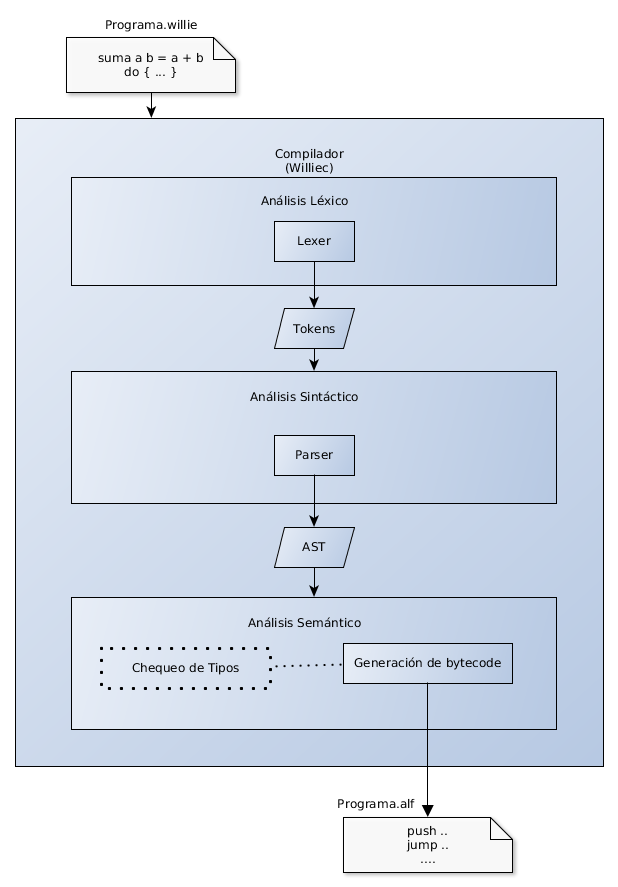
\includegraphics[width=0.9\textwidth]{graphs/compiler.png}
\label{fig:compiler}
\end{center}
\end{figure}




\subsection{Análisis Léxico}
  La primera etapa se llama análisis léxico, en esta se lee el código
  fuente en lenguaje \frob{} (.willie) y lo transforma en una
  lista de lexemas.

  Un lexema puede ser una palabra reservada (ej: \texttt{do}),
  un valor (ej: $19$), un identificador (eg: \texttt{distance}) o un símbolo reservado (eg: \texttt{+}).

  Para representar los lexemas, se utiliza la herramienta \textit{UU.Scanner}
  \cite{uuparser} que estandariza los mismos en el tipo de
  datos \texttt{Token}.
  Usando \textit{Alex} se procesa el código fuente, se reconocen los lexemas y se retorna una lista de tipo \texttt{[Token]}.

  La etapa se puede resumir en la implementación de la función \texttt{tokenize}.

\begin{Verbatim}
  tokenize :: String -> String -> [Token]
\end{Verbatim}




\subsection{Análisis Sintáctico}
  La segunda fase del compilador, recibe la lista de lexemas (\texttt{[Token]}) y
reconoce el lenguaje, generando un árbol de
sintaxis abstracta (\emph{AST}\footnote{Del inglés Abstract Syntax Tree}).

  Para reconocer la gramática se implementó un parser recursivo descendente.
  Utilizando la herramienta \textit{UU.Parser} \cite{uuparser}, se definió un tipo de datos
  \texttt{TokenParser a} que representa un parser que recibe una secuencia de lexemas de tipo \texttt{Token}
  y retorna un \emph{AST} de tipo \texttt{a}.

  \begin{Verbatim}
  type TokenParser a = Parser Token a
  \end{Verbatim}

  \textit{UU.Parser} define un conjunto de combinadores de parsers y utilizándolos se construyen parsers
  complejos a partir de parsers simples.

  Para representar el \emph{AST} se utiliza una gramática de atributos.
  Una gramática de atributos es como una gramática libre de contexto, pero agrega semántica a la misma.
  Para el análisis sintáctico, la semántica no es utilizada, pero será usada en la próxima etapa.

  El sistema de gramáticas de atributos
  \textit{UUAG}\cite{uuag} fue usado para la implementación.


  Se define un tipo de datos \texttt{Root} que representa la raíz del árbol.

  \begin{Verbatim}
  data Root
    | Root
      decls :: Decls
      dodecls :: Dodecls
  \end{Verbatim}

  El mismo tiene un único constructor \texttt{Root\_Root} que recibe un árbol de tipo
  \texttt{Decls} que representa las declaraciones, y un árbol de tipo \texttt{Dodecls} que
  representa el bloque \texttt{do}.

  Para crear el \emph{AST} usando \textit{UU.Parser} se define el parser \texttt{pRoot}:

  \begin{Verbatim}
  pRoot :: TokenParser Root
  pRoot
    = Root_Root <$> pDecls <*> pDodecls
  \end{Verbatim}

  El cuál asume definido un parser de declaraciones \texttt{pDecls} y un parser
  del bloque \texttt{do} (\texttt{pDodecls}).
  
  \begin{Verbatim}
  pDecls :: TokenParser Decls

  pDodecls :: TokenParser Dodecls
  \end{Verbatim}

  El combinador ``$\langle * \rangle$'' \cite{uuparsing:piriapolis} se utiliza para
  combinar dos parser y resolver producciones de largo 2 en una gramática,
  en este caso reconocer primero la lista de declaraciones de funciones, y
  luego el bloque \texttt{do}.
  El tipo del combinador es:

  \begin{center}
    $(\langle*\rangle) :: \texttt{Parser}\ s\ a \rightarrow \texttt{Parser}\ s\ b \rightarrow \texttt{Parser}\ s\ (a, b)$
  \end{center}

  El combinador ``$\langle \$ \rangle$'' se utiliza para aplicar una
función al resultado de un parser, en éste caso la función es aplicar
el constructor \texttt{Root\_Root}.

  Para construir el parser completo, se va refinando sucesivamente
en parsers mas específicos, hasta construir completamente el \emph{AST}.
  En el apéndice \ref{appendix:parser} se encuentra código del parser
implementado.



\subsection{Análisis Semántico}
\label{subsection:implementation:semantics}
  Para la última etapa se utiliza la gramática de atributos para definir
semántica sobre el \emph{AST}.

Las gramáticas de atributos (\emph{Attribute Grammars}
\cite{attributegrammars} \cite{uuag}) simplifican
la tarea de escribir catamorfismos.
Un catamorfismo es una función análoga a la función de alto orden
\texttt{foldr} pero aplicada sobre cualquier tipo de datos recursivo.

  De ésta manera se pueden definir atributos sintetizados,
  heredados o mixtos en el \emph{AST}.

  Los atributos sintetizados son valores que se distribuyen desde las
hojas hacia la raiz del \emph{AST}, y los heredados aquellos que
se distribuyen desde la raiz hacia las hojas.

  Uno de dichos atributos será el código en bajo nivel, la salida
de esta etapa.

  Se implementó una gramática de atributos usando \textit{UUAG}, y con
  el compilador de gramáticas \textit{UUAGC}\cite{uuagc} se
  compiló a \haskell{}.

  El compilador \textit{UUAGC} toma la gramática y construye los
  catamorfismos necesarios para procesar todos los atributos.

  Construir el compilador, se reduce a obtener una secuencia de atributos
  sobre el \textit{AST} que sirven para generar el código \alf{}.

  Por ejemplo para construir el código de un programa, la raiz
  del \textit{AST} está dada por el tipo de datos \texttt{Root}.

\begin{Verbatim}
data Root
  | Root
      decls :: Decls
      dodecls :: Dodecls
\end{Verbatim}

  Se puede definir el código como la concatenación del código de
  las declaraciones del bloque \texttt{do}, una instrucción \texttt{halt}
  y el código de las declaraciones de funciones (\texttt{Decls}).

  Para ésto se define un atributo sintetizado (\texttt{syn})
  llamado \texttt{code}.


\begin{Verbatim}
set All = Root Decls Decl Dodecls Dodecl Expr
attr All syn code use {++} {[]} :: BC

sem Root
  | Root
    lhs.code = @dodecls.code ++ [Thalt] ++ @decls.code
\end{Verbatim}

  Utilizando la palabra clave \texttt{Set} se define el conjunto \texttt{All}
de elementos para los que se definirá el atributo.
  
  En la definición del atributo, se especifica que en caso de no haber
una regla específica, se calcula usando la concatenación \texttt{++}
y como atributo por defecto toma \texttt{[]}. A ésto se le llama
\textit{use rule}.

  \begin{Verbatim}
  attr All syn code use {++} {[]} :: BC
  \end{Verbatim}

  Por ejemplo para la definición de la lista de declaraciones:

\begin{Verbatim}
type Decls = [Decl]
\end{Verbatim}

  No es necesario especificar que el código se obtiene concatenando sus
  partes ya que se infiere automáticamente usando la regla anterior.


  Para poder generar el código de todo el programa, es necesario
  calcular otros atributos previos.
  Se necesita saber la posición en la que quedarán las funciones para
  poder tener una referencia a ellas.
  Para saber la posición, es necesario calcular el largo del código
  antes de tener el código.

  Para ésto se definió un atributo sintetizado \texttt{len} que contiene
  el largo que tendrá cada bloque luego de traducido
  a código, pero sin llegar a traducirlo.

  También se definió un atributo \texttt{pos} que indica en que posición
  estará ubicado el código que se genere para cada producción de la
  gramática.
  El atributo \texttt{pos} es un atributo heredado (\texttt{inh}) en
  el \textit{AST}.

  Por ejemplo en \texttt{Root}, se utiliza el atributo \texttt{len} 
  de las declaraciones del bloque \texttt{do} para saber a partir
  de que posición \texttt{pos} estarán ubicadas las declaraciones
  de funciones.

\begin{Verbatim}
attr All syn code use {++} {[]} :: BC
         syn len use {+} {0} :: Int
         inh pos :: Int
 
sem Root
  | Root
      lhs.code = @dodecls.code ++ [Thalt] ++ @decls.code
      dodecls.pos = 0
      decls.pos = @dodecls.len + 1
\end{Verbatim}

  Utilizando el atributo \texttt{pos}, se puede saber en que posición
  estará cada función en el código generado.
  Para tener la posición de todas las funciones se utiliza un atributo
  encadenado (\texttt{chn}) llamado \texttt{labels},
  es heredado pero también es sintetizado.
  Por ejemplo al declarar una función, se agrega la posición \texttt{pos}
  asociada al nombre de la misma.

\begin{Verbatim}
sem Decl
  | Function
      lhs.code = @body.code ++ [Tret]
      lhs.len = @body.len + 1
      lhs.labels = addLabel @name @lhs.pos @lhs.labels
\end{Verbatim}

  El atributo contiene un mapa que dado un nombre de una función retorna
  la posición de la misma, \texttt{labels} recolecta la posición de todas
  las funciones.
  Luego otro atributo \texttt{labelMap} se declara como heredado \texttt{inh}
  y se le asigna en \texttt{Root} el valor de \texttt{labels},
  \texttt{labelMap} se usa para distribuir el mapa
  completo en todo el \textit{AST}.

\begin{Verbatim}
sem Root
  | Root
      decls.labels = emptyLabelMap
      decls.labelMap = @decls.labels
      dodecls.labelMap = @decls.labels
\end{Verbatim}

  Por último un atributo \texttt{env} encadenado recolecta las declaraciones
  de identificadores, a cada identificador de señal le asigna un número
  entero único y mantiene la lista de las variables en el alcance (scope)
  dentro de una función. 
  Luego que el atributo \texttt{env} recolecta todas las declaraciones,
  el resultado es distribuido con el atributo heredado \texttt{envInh}.

\begin{Verbatim}
sem Root
  | Root
      decls.env = emptyEnv
      dodecls.env = emptyEnv
      dodecls.envInh = @dodecls.env
\end{Verbatim}

  Usando todos éstos atributos se genera el código para cada producción
  de la gramática, y el atributo \texttt{code} se puede calcular.

  Se definió un módulo \texttt{Bytecode} que abstrae el código
  de máquina en un tipo \texttt{OpCode} y define funciones para 
  exportarlo como texto o en formato binario.

% TODO(Marcos): Agregar un diagrama con los modulos, indicando que es
% generado y que importa a que.

  Al compilar la gramática usando \textit{UUAGC} se obtiene un módulo
  en lenguaje \texttt{Haskell} que expone la función \texttt{code\_Syn\_Root}
  y deja accesible el código resultado como una lista de
  tipo \texttt{[OpCode]}.

  Utilizando el módulo \texttt{Bytecode}, el código se obtiene y 
  escribe en un archivo (.alf) terminando el proceso de compilación.



\section{Máquina virtual}
  
  
  La máquina virtual será la encargada de recibir el bytecode creado por
el compilador, e interpretarlo en la plataforma que esté ejecutando.
  A diferencia del compilador, es necesario implementar una máquina virtual
para cada arquitectura objetivo.\\

  Por ejemplo, para ejecutar programas en un robot
  con un procesador \emph{arduino}, debe
  existir una implementación de la máquina para ese modelo
  de \emph{arduino}.

  Al momento de implementar la máquina, se tomará en cuenta ésto para
  factorizar partes en común y sólo implementar por arquitectura, las
  partes que realmente sean diferentes como ser la comunicación con
  los periféricos de entrada/salida y las llamadas al sistema.


TODO: Describir el diseño de la máquina virtual.

  La máquina virtual va a ser basada en stack. Ésto significa
que las operaciones van a tomar sus argumentos del stack y
colocar resultados en el mismo.



\chapter{Casos de estudio}

  En esta sección veremos un caso de estudio usado para verificar la
implementación.
  El problema fue tomado de la competencia SumoUY \cite{sumouy}, el mismo
fue el desafío planteado a escolares en el año 2013.

\section {Problema}

  Se desea implementar un robot autónomo móvil que sea capaz de
hacer la entrega de un pedido en una casa determinada.
  El mismo debe moverse por un escenario e identificar las casas.
  Para recorrer la ruta de entrega, podrá valerse de una línea negra
que representará la calle de la ciudad.

  Las casas estarán ubicadas a un lado de la calle. En el recorrido
se encuentran varias casas, el robot deberá entregar un pedido
en la quinta casa por la que pase.

  El robot deberá pasar por alto las casas anteriores y
al llegar a la casa objetivo debe detenerse totalmente.

  Para probar la solución, se armará un escenario que consiste de
un piso blanco con una línea negra que puede tener curvas.

  Al lado derecho de la línea se ubicarán cajas a menos de 30
centímetros representando las casas.

\section {Solución}

  Se armó un robot móvil que cuenta con 3 sensores:

\begin{itemize}
\item Sensor de grises izquierdo
\item Sensor de grises derecho
\item Sensor de distancia apuntando hacia la derecha
\end{itemize}

  Y 2 actuadores:

\begin{itemize}
\item Motor izquierdo
\item Motor derecho 
\end{itemize}

  El robot utilizará los sensores de grises para mantenerse sobre
la línea y el sensor de distancia para saber cuándo está frente
a una casa.

  Con los motores se moverá hacia adelante inicialmente, e irá corrigiendo
  su dirección desacelerando el motor del lado que se salga de la línea.

  Durante el trayecto contará las casas, y se detendrá cuando la cuenta
llegue al valor 5.

  En el siguiente diagrama, se puede ver gráficamente de que forma
se combinan los eventos, para lograr nuestro objetivo:

\begin{figure}[hbtp]
\begin{center}
\caption{Diagrama del caso de estudio}
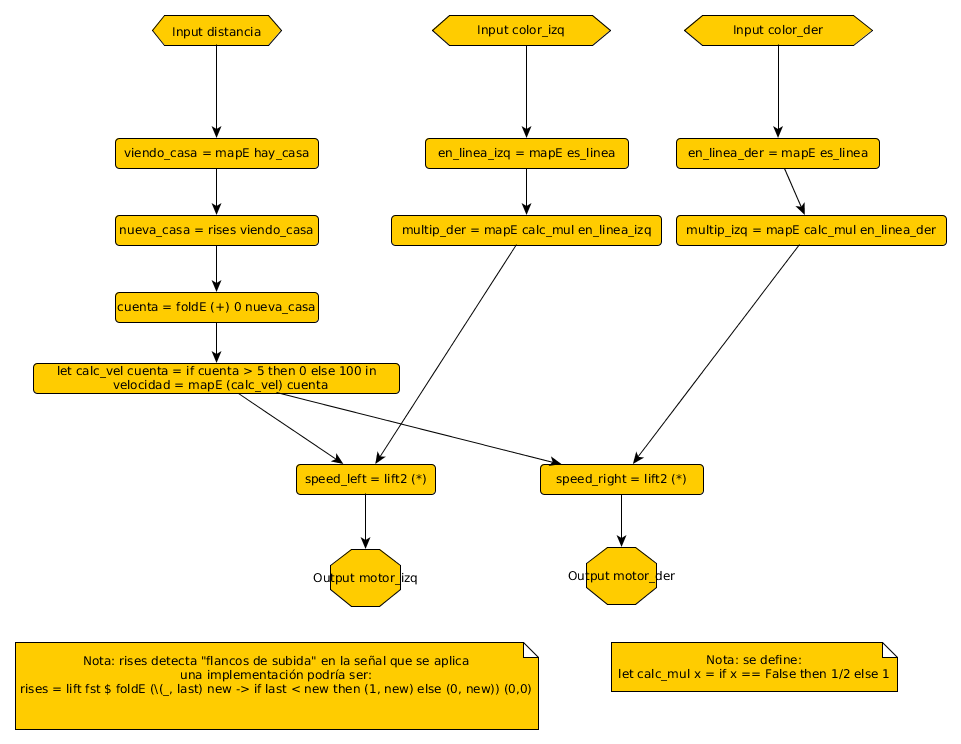
\includegraphics[width=0.9\textwidth]{graphs/delivery.png}
\label{fig:delivery}
\end{center}
\end{figure}

  Luego se llega a la implementación en el lenguaje \frob :

\begin{verbatim}

INPUT_DISTANCE = 1
INPUT_COLOR_LEFT = 2
INPUT_COLOR_RIGHT = 3
OUTPUT_ENGINE_LEFT = 1
OUTPUT_ENGINE_RIGHT = 2

MIN_DISTANCE = 100
MIN_GREY = 50

hay_casa d = if (d < MIN_DISTANCE) then 1 else 0
distinto a b = if (a /= b) then 1 else 0
and a b = if (a && b) then 1 else 0

velocidad_casa num = if (num >= 5) then 0 else 100

suma a b = (a + b)

color_a_vel gris = if (gris > MIN_GREY) 1 else 1/2

multiplicar a b = (a * b)

do {
    distance <- read INPUT_DISTANCE,
    color_izq <- read INPUT_COLOR_LEFT,
    color_der <- read INPUT_COLOR_RIGHT,

    viendo_casa <- lift hay_casa distance,
    cambio <- folds distinto viendo_casa,
    nueva_casa <- lift2 and viendo_casa cambio,
    cuenta <- folds suma 0 nueva_casa,
    velocidad <- lift velocidad_casa cuenta,

    multip_izq <- lift color_a_vel color_izq,
    multip_der <- lift color_a_vel color_der,

    speed_left <- lift2 multiplicar velocidad multip_izq,
    speed_right <- lift2 multiplicar velocidad multip_der,

    output MOTOR_IZQ speed_left,
    output MOTOR_DER speed_right
}

\end{verbatim}

\section {Conclusiones del caso}




\chapter{Conclusiones}

Intro .... que se hizo, puntos a favor, etc..

\section{Trabajo futuro}

El principal trabajo futuro sería ...

Sería muy útil contar con una funcionalidad de depuración, la cuál
mostrara dependiendo del tiempo los valores de cada fuente de eventos.

Una opción es comunicar mediante el puerto serial el valor de cada
señal al cambiar, y mostrarlo en una interfaz web como la que provee
RXMarbles (ver \cite{rxmarbles}). 
El lenguaje Elm provee de una herramienta que permite viajar en el 
tiempo, modificar y mostrar la ejecución de un programa, en nuestro
caso no sería posible modificar lo que el robot físico realiza, pero
si sería útil ver en la línea de tiempo que valores tomaron sus
señales. (ver \cite{elmdebug})



% Bibliografia
\cleardoublepage
\addcontentsline{toc}{chapter}{Bibliografía}

%\begin{thebibliography}{99}
%\bibitem{katoen} \emph{Principles of Model Checking}.\\
 Christel Baier y Joost-Pieter Katoen.\\
 The MIT Press, 2008.

% http://conal.net/papers/frp.html
%@InProceedings{ElliottHudak97:Fran,
%  title        = {Functional Reactive Animation},
%  url          = {http://conal.net/papers/icfp97/},
%  author       = "Conal Elliott and Paul Hudak",
%  booktitle    = "International Conference on Functional Programming",
%  year         = 1997
%}

% Yampa, Arrows and Robots.

%@InProceedings{Peterson99:LambdaInMotion,
%  author       = {John Peterson and Paul Hudak and Conal Elliott},
%  title        = {Lambda in Motion: Controlling Robots with {Haskell}},
%  url          = {http://haskell.org/frob/padl99/padl99.ps},
%  booktitle    = {Practical Aspects of Declarative Languages},
%  year         = 1999
%}
% http://cs.brown.edu/research/pubs/techreports/reports/CS-03-20.html

% Informal pero ayudo:
% https://gist.github.com/staltz/868e7e9bc2a7b8c1f754
%
% Rx, Bacon.js, 
%
% Para debug muy bueno: (con RX es este)
% https://github.com/jaredly/rxvision
% http://lambdor.net/?p=44

% Elm Creator:
% Evan Czaplicky "Controlling Time and Space. https://www.youtube.com/watch?v=Agu6jipKfYw a video can be a reference? "
% elm-lang.org/papers/concurrent-frp.pdf (evan czaplicky thesis)
% SEGUIR CON:::j
% https://vimeo.com/77164337

\bibitem{python} Sitio web de \emph{Python 2.7}:\\
 \url{http://docs.python.org/2/}\\
 Último acceso: 31/10/2013.

\bibitem{gml} Sitio web de \emph{GraphML File Format}:\\
 \url{http://graphml.graphdrawing.org/}\\
 Último acceso: 31/10/2013.


\bibliographystyle{unsrt}
\bibliography{Informe}

%\end{thebibliography}


% Apendices
\appendix
\cleardoublepage
\addappheadtotoc
\appendixpage

\chapter{Apéndice}

\section{Manual de usuario}


  Para utilizar el compilador, dado un archivo \textit{Ejemplo.willie}, se
ejecuta:

\begin{Verbatim}
> williec < Ejemplo.willie > Ejemplo.alf
\end{Verbatim}



El código de la máquina virtual está en el directorio
  /src/alfvm, para compilarlo se ejecuta:
\begin{verbatim}
  > cd src/alfvm
  > make
\end{verbatim}




\section{Manual de Referencia}


\subsection{Instrucciones de bajo nivel}

  A continuación se presenta el resto de las instrucciones
de bajo nivel y pseudocódigo indicando su semántica.

\begin{itemize}

\item \texttt{halt}

  Detiene el hilo de ejecución actual.

  \texttt{ip = 0} 

\item \texttt{call function}

  Invoca la funcion $function$.
  Se asume que los parámetros están en el stack.

\item \texttt{ret}

  Toma el resultado de una función del tope del stack,
  limpia el espacio ocupado por la función,
  y deja el resultado en el nuevo tope del stack.

  \texttt{value = stack.pop()}

  \texttt{stack.pop\_frame();}

  \texttt{ip = code[stack.pop()]}

  \texttt{fp = stack.pop()}

  \texttt{stack.pop\_args()}

  \texttt{stack.push(value)}

\item \texttt{load\_param inm}

  \texttt{a = stack.get\_arg(inm)}

  \texttt{stack.push(a)}

\item \texttt{jump}

  \texttt{goto position}

\item \texttt{jump\_false position}

  \texttt{a = stack.pop()}

  \texttt{if not a: goto position}

\item \texttt{cmp\_eq}

  \texttt{a = stack.pop()}

  \texttt{b = stack.pop()}

  \texttt{stack.push(a == b)}

\item \texttt{cmp\_neq}

  \texttt{a = stack.pop()}

  \texttt{b = stack.pop()}

  \texttt{stack.push(a != b)}

\item \texttt{cmp\_gt}

  \texttt{a = stack.pop()}

  \texttt{b = stack.pop()}

  \texttt{stack.push(a > b)}

\item \texttt{cmp\_lt}

  \texttt{a = stack.pop()}

  \texttt{b = stack.pop()}

  \texttt{stack.push(a < b)}

\item \texttt{add}

  \texttt{a = stack.pop()}

  \texttt{b = stack.pop()}

  \texttt{stack.push(a + b)}

\item \texttt{sub}

  \texttt{a = stack.pop()}

  \texttt{b = stack.pop()}

  \texttt{stack.push(a - b)}

\item \texttt{div}
  
  \texttt{a = stack.pop()}

  \texttt{b = stack.pop()}

  \texttt{stack.push(a / b)}

\item \texttt{mul}

  \texttt{a = stack.pop()}

  \texttt{b = stack.pop()}

  \texttt{stack.push(a * b)}

\item \texttt{op\_and}

  \texttt{a = stack.pop()}

  \texttt{b = stack.pop()}

  \texttt{stack.push(a and b)}

\item \texttt{op\_or}

  \texttt{a = stack.pop()}

  \texttt{b = stack.pop()}

  \texttt{stack.push(a or b)}

\item \texttt{op\_not}

  Coloca un valor constante en el stack.

  \texttt{stack.push(word)}

\item \texttt{push word}

  Coloca un valor constante en el stack.

  \texttt{stack.push(word)}

\item \texttt{pop}

  Elimina el tope del stack.

  \texttt{stack.pop()}

\item \texttt{dup}

  Duplica el tope del stack.

  \texttt{stask.push(stack.tos())}

\item \texttt{store inm}

  Guarda el tope del stack en la variable $inm$.

  \texttt{var[inm] = stack.pop()}

\item \texttt{load inm}

  Carga la variable $inm \in {0..255}$ en el stack.

  \texttt{stack.push(var[inm])}

\end{itemize}




%
%\chapter{Archivos \textit{GraphML}}
%Como se mencionó anteriormente se utilizó el formato de archivo \textit{GraphML} para
 representar los sistemas de transiciones.
Los estados son representados por el elemento \texttt{node} mientras que las transiciones
 son representadas por el elemento \texttt{edge}.

El formato \textit{GraphML} no establece como representar las etiquetas tanto en los nodos
 como en las aristas.
Para esto existe el atributo \texttt{data}, que proporciona flexibilidad
 para agregar atributos no contemplados por el formato.
Esto tiene un desventaja, y es que los atributos no contemplados por el formato no se
 representan de forma estándar, y por lo tanto su representación depende del editor
 utilizado.
En este caso el editor utilizado es \textit{yEd}.

Para los estados se guarda la siguiente información:
\begin{itemize}
\item Identificador

Este valor se guarda en el atributo \texttt{id} de cada nodo.
Es el identificador del estado, por lo que debe ser único.

Cuando se genera un sistema de transiciones mediante el verificador este genera los identificadores
 de cada estado automáticamente.

\item Proposiciones

Representan el conjunto de las proposiciones válidas en cada estado.

Se guardan en el atributo \texttt{y:NodeLabel}.
Este atributo es se encuentra dentro del atributo \texttt{data}, ya que no se encuentra
 especificado en el formato.

En caso de haber varias proposiciones, estas deben estar separadas por comas.

\end{itemize}

Además de esta información se debe indicar cuales son los estados iniciales.

Para las transiciones se debe guardar la siguiente información:
\begin{itemize}
\item Origen

Representa el estado de origen de la transición. Se guarda en el atributo \texttt{source}.

\item Destino

Representa el estado de destino de la transición. Se guarda en el atributo \texttt{target}.

\item Acción

Representa la acción que corresponde al cambio de estado.

Se guardan en el atributo \texttt{y:EdgeLabel}.

Este atributo es se encuentra dentro del atributo \texttt{data}, ya que no se encuentra
 especificado en el formato.

\end{itemize}

El parser de \textit{GraphML} a sistemas de transiciones se encuentra implementado en
 el objeto \texttt{ParserGraphML} del paquete \textit{Sistemas de transiciones}.

Como se mencionó anteriormente hay atributos que no están especificados en el formato y
 por lo tanto su interpretación depende del editor utilizado. Estos atributos son especificados
 en el parser mediante sub clases.
En este caso se utiliza el \textit{yEd Graph Editor}, para el cual fue implementado el objeto
 \texttt{ParserGraphML\_yEd}.
Este objeto es un parser de \textit{GraphML} que además interpreta la información dentro del
 atributo \texttt{data} como las etiquetas de los estados y transiciones.

A continuación se muestra un ejemplo de un sistema de transiciones y su correspondiente
 representación en \textit{GraphML}.

\paragraph{Ejemplo de sistema de transiciones en \textit{GraphML}} 





% Termina el documento
\end{document}
